\pattern{Blackboard}
\begin{summary}
a behavioural design pattern for systems that need to integrate multiple
individually specialized computation modules to solve complex problems where
information is ambiguous, and the path to the solution is not known in advance.
Its architectural topology can be separated into 3 main sub-categories: the
blackboard, the knowledge sources, and the controller, as shown in Figure 1. In
general, the blackboard is a shared memory space holding information
representing the state of a problem on which knowledge sources (KS) will
operate when recruited by the controller, applying their specialized knowledge
to contribute to the ultimate formation of a solution. This cooperative process
will be discussed in more detail in the next sections.

The blackboard architecture is ideal for solving problems where information is
ambiguous or the path to the solution is not known in advance. The blackboard
is a shared memory space that is responsible for acting as a hub for all
streamed data, solutions, and partial solutions. The KSs, also called “experts”
or “agents”, are responsible for performing very specific tasks to contribute
to the final solution. A KS is generally used to determine if the problem has
been solved or solved enough. Not all KSs need to contribute to a solution or
to be run in order to sufficiently find the solution to a problem. Controllers
are used to orchestrate the KSs. Many algorithms can be used with the
controller to help optimize the execution of KSs.

The blackboard is a shared memory space. This means that all the information
streamed into the system or processed by the KSs will persist in this shared
space, fully accessible by all components in the system. At any given point in
time, the blackboard is not required to have the full solution to the problem
the system is built for. Instead, it will hold partial solutions to smaller
subproblems solved and, eventually, due to the non-deterministic nature of the
control process, will contain a solution that is deemed viable to a certain
degree of precision. The KSs are the “experts” responsible for processing and
contributing to the solution as a whole.

\end{summary}

\subsubsection{Implementation}

Knowledge sources, also called agents, can be thought of as specialised
“experts” in being able to perform very specific tasks. From the perspective of
the blackboard, the KSs form a panel of individuals, unaware of each other, who
will contribute their niche resources to advance the problem toward an
acceptable solution state. Incidentally, this decoupling of resources makes
blackboard architecture very modular, making reuse of KSs very easy for new
blackboard implementations. Collectively, the incremental solutions processed
and reposted to the blackboard by the KSs will converge on a solution. One of
the KSs may be responsible for marking a solution presented on the blackboard
as “viable”. The degree of the viability of a solution depends entirely on the
problem and the defined criteria for an acceptable solution.

In some implementations of this architecture, a controller is not even
necessary. The KSs evaluate the information presented on the blackboard and, if
able, they process them on their own, possibly editing metadata associated with
the information they want to process to keep track of the problem state.
However, the purpose of this pattern is to provide an architectural framework
that is capable of solving complex, non-deterministic control problems. This
means that the KSs may not necessarily run linearly; they can run in parallel.
Optimization is at the root of control problems where resource allocation in
parallel computation is necessary to most efficiently compute a solution to a
problem. This is where a controller comes into the picture to help address the
optimization problem.

The controller is responsible for assigning tasks to the KSs to process
information on the blackboard. The goal is to converge on a solution that is
considered acceptable for the problem. The way in which the controller,
blackboard, and KSs communicate (i.e. event-based, polling,
publisher-subscriber, etc.) is less important than the roles they play, and
thus not rigidly defined in the architecture.

% \comparison{\begin{itemize}

% \end{itemize}
% }{\begin{itemize}

% \end{itemize}}

\begin{nfps}
\item[Reusable] A single KS can be used by multiple blackboards. Since they are independent from each other, they can be reused in other blackboard architecture problems.

\item[Scalable] Because of the flexibility of the KSs it is easy to add and
    remove them. If we wish to have a better solution, adding agents could
    help. The controller just needs to be modified to take into consideration
    the changes. Overall, if the system requires more processing power, then
    additional agents can be added to create a better throughput.

\item[Robust] If a KS fails to complete its task or is unavailable, then a
    solution might still be found thanks to the other KSs. Note that it might
    not be as optimal or complete.

\end{nfps}

\begin{center}
    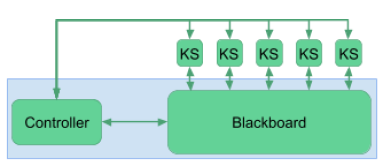
\includegraphics[width=0.4\textwidth]{./blackboard}
\end{center}
